\documentclass[tikz,border=2pt]{standalone}
\usepackage{amsmath,amssymb}
\usepackage{pgfplots}
\pgfplotsset{compat=1.18}
\usetikzlibrary{arrows.meta}

\begin{document}
% Standardizing X ~ N(5, 2^2): subtracting mu = 5 slides the curve to 0, dividing by sigma = 2
% squeezes it to unit spread, giving Z ~ N(0, 1). The same two steps work for any X.
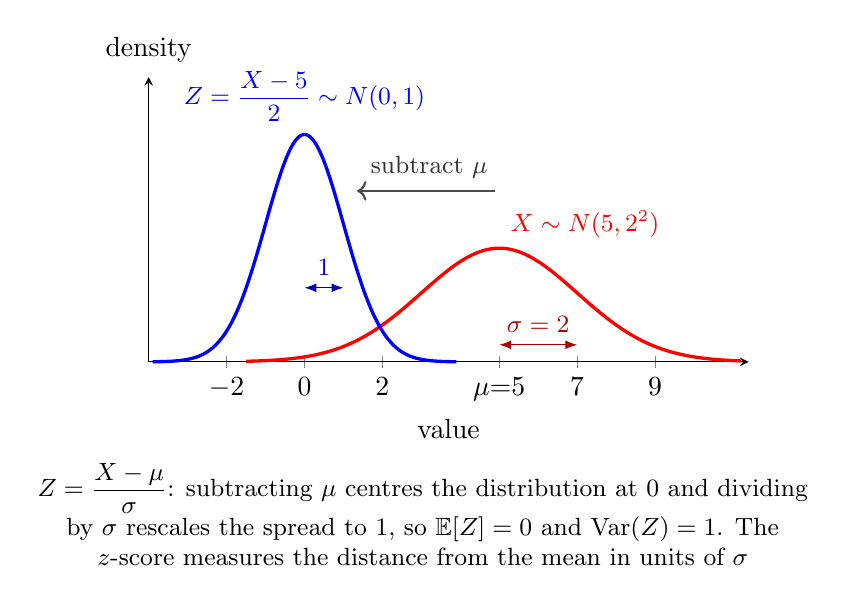
\begin{tikzpicture}
	\begin{axis}[
		axis lines=left, xmin=-4, xmax=11.4, ymin=0, ymax=0.5,
		xtick={-2,0,2,5,7,9}, xticklabels={$-2$,$0$,$2$,$\mu{=}5$,$7$,$9$}, ytick=\empty,
		xlabel={value}, ylabel={density}, ylabel style={rotate=-90, anchor=south, at={(axis description cs:0,1.02)}},
		samples=200, smooth, width=9.2cm, height=5.2cm, clip=false
		]
		\addplot[red, very thick, domain=-1.5:11.2] {exp(-(x-5)^2/8)/(2*sqrt(2*pi))};
		\addplot[blue, very thick, domain=-3.9:3.9] {exp(-x^2/2)/sqrt(2*pi)};
		\node[blue, anchor=south, font=\small] at (axis cs:0,0.405) {$Z=\dfrac{X-5}{2}\sim N(0,1)$};
		\node[red, anchor=south, font=\small] at (axis cs:7.2,0.2) {$X\sim N(5,2^2)$};
		\draw[->, gray!60!black, thick] (axis cs:4.9,0.3) -- (axis cs:1.35,0.3);
		\node[gray!40!black, anchor=south, font=\small] at (axis cs:3.2,0.305) {subtract $\mu$};
		\draw[{Latex[length=1.5mm]}-{Latex[length=1.5mm]}, red!70!black] (axis cs:5,0.03) -- (axis cs:7,0.03);
		\node[red!70!black, anchor=south, font=\small] at (axis cs:6,0.035) {$\sigma=2$};
		\draw[{Latex[length=1.5mm]}-{Latex[length=1.5mm]}, blue!70!black] (axis cs:0,0.13) -- (axis cs:1,0.13);
		\node[blue!70!black, anchor=south, font=\small] at (axis cs:0.5,0.135) {$1$};
	\end{axis}
	\node[anchor=north, font=\small, align=flush center, text width=9.8cm] at ([yshift=-2pt]current axis.outer south) {$Z=\dfrac{X-\mu}{\sigma}$: subtracting $\mu$ centres the distribution at $0$ and dividing by $\sigma$ rescales the spread to $1$, so $\mathbb{E}[Z]=0$ and $\operatorname{Var}(Z)=1$. The $z$-score measures the distance from the mean in units of $\sigma$};
\end{tikzpicture}
\end{document}
